\newpage
\section{Valutazione dei modelli}
Quasi sempre quando si addestra un modello di ML, occorre un modo per valutare le 
sue prestazioni.

\subsection{La Matrice di confusione}
Una matrice di confusione (o matrice di errore) è un metodo di visualizzazione 
per i risultati dell'algoritmo di classificazione. Più specificamente, 
è una tabella che suddivide il numero di istanze di verità di base di una 
classe specifica rispetto al numero di istanze di classe previste.
In una matrice di confusione, le colonne rappresentano i valori previsti di una 
data classe, mentre le righe rappresentano i valori effettivi 
(ad esempio, le verità di base) di una data classe, o viceversa.
Questa struttura a griglia è uno strumento utile per visualizzare l'accuratezza 
della classificazione dei modelli. In quanto permette di visualizzare 
il numero di previsioni corrette e previsioni errate per tutte le classi una 
accanto all'altra
\cite{Confusion_Matrix_e_metrics1,Confusion_Matrix_e_metrics2}.

Un modello di matrice di confusione standard per un classificatore 
binario può essere simile a:

\begin{figure}[H]
    \centering
    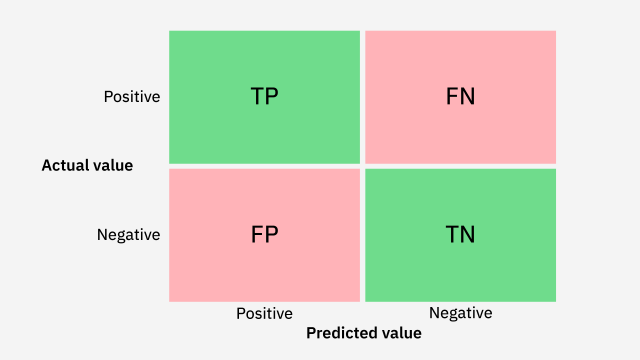
\includegraphics[width=0.60\textwidth]{Immagini/Grafici/esempio_MC_1.png}
    \caption{Esempio di una matrice di confusione per classificazione binaria
    \cite{Confusion_Matrix_e_metrics1} .}
\end{figure}

La casella in alto a sinistra fornisce il numero di veri positivi (TP), ovvero 
il numero di previsioni corrette per la classe positiva. Il riquadro sottostante è 
rappresentato dai falsi positivi (FP), ovvero quei casi di classe negativa erroneamente 
identificati come casi positivi. In statistica, questi sono anche chiamati errori 
di tipo I. La casella in alto a destra indica il numero di falsi negativi (FN), 
i casi effettivamente positivi erroneamente previsti come negativi. Infine, nella 
casella in basso a destra viene visualizzato il numero di veri negativi (TN), 
ovvero le istanze effettive della classe negativa previste con precisione. 
Sommando ciascuno di questi valori si otterrebbe il numero totale di previsioni 
del modello \cite{Confusion_Matrix_e_metrics1,Confusion_Matrix_e_metrics2}.

% Naturalmente, questo modello è per un rudimentale problema di classificazione 
% binaria. La matrice di confusione può visualizzare i risultati anche per 
% problemi di classificazione multiclasse. 
% Ad esempio, immaginiamo di sviluppare un 
% modello di classificazione delle specie come parte di un programma di conservazione 
% della vita marina. Il modello prevede le specie ittiche. 
\newpage
Una matrice di confusione può essere utilizzata anche per problemi di 
classificazione multiclasse. 
%di questo tipo può essere simile alla seguente:

\begin{figure}[H]
    \centering
    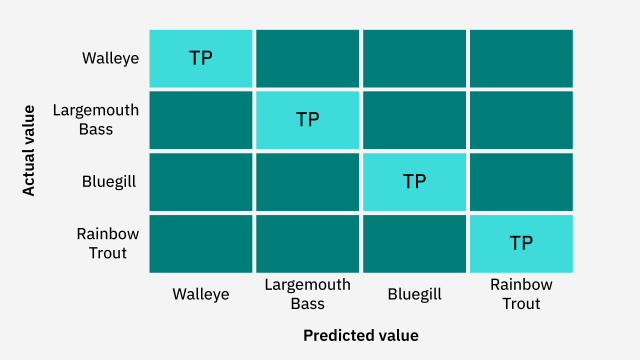
\includegraphics[width=0.70\textwidth]{Immagini/Grafici/esempio_MC_2.png}
    \caption{Esempio di una matrice di confusione per classificazione multi classe}
    %\label{fig:rappresentazione dell'IA, ML e DL}
    %Figura 2.1: Esempio schematico di un neurone
\end{figure}

Tutte le caselle diagonali indicano i veri positivi previsti. 
Le altre caselle forniscono le quantità per i falsi positivi, i falsi 
negativi ed i veri negativi a seconda della classe che si sceglie di mettere a fuoco.
La matrice di confusione può servire a calcolare diverse metriche di valutazione, 
come per esempio il tasso di errore, l’accuratezza, la precisione, 
il richiamo o sensibilità (Recall) e l’F1-score.
Mettendo la matrice di confusione e le metriche ad essa associate sotto osservazione, 
è possibile identificare le aree in cui il modello presenta criticità. 
Così è possibile adottare misure specifiche per aumentare la precisione 
delle previsioni \cite{Confusion_Matrix_e_metrics1,Confusion_Matrix_e_metrics2}.

\subsection{L'accuratezza}

% L’accuratezza rappresenta la percentuale di predizioni corrette 
% rispetto al totale delle predizioni. L'accuratezza varia da 0 (scenario peggiore) 
% a 1 (previsione migliore).

L'accuratezza rappresenta la percentuale di predizioni corrette 
rispetto al totale delle predizioni effettuate. Questo valore 
varia da 0, che rappresenta lo scenario peggiore in cui tutte le predizioni sono errate, 
a 1, che corrisponde alla massima accuratezza con tutte le predizioni corrette.
L'accuratezza si calcola utilizzando la seguente formula:

\begin{equation}
    \text{ACC} = \frac{\text{Casi corretti}}{\text{Numero totale di casi}}=\frac{TP + TN}{TP+TN+FP+FN}
\end{equation}

Tuttavia, l'accuratezza del modello non è una metrica di valutazione completamente 
informativa per i classificatori. Immaginiamo, ad esempio, di eseguire un 
classificatore su un set di dati di 100 istanze. La matrice di confusione 
del modello mostra solo un falso negativo e nessun falso positivo; 
il modello classifica correttamente ogni altra istanza di dati. 
Pertanto, il modello ha una precisione del 99\%. 
Sebbene apparentemente desiderabile, l'elevata precisione non è di per sé 
indicativa di eccellenti prestazioni del modello. 
Ad esempio, supponiamo che il nostro modello miri a classificare malattie 
altamente contagiose. Questa errata classificazione dell'1\% rappresenta un 
rischio enorme. Pertanto, è possibile utilizzare altre metriche di valutazione 
per fornire un quadro migliore delle prestazioni dell'algoritmo di classificazione
\cite{Confusion_Matrix_e_metrics1,Confusion_Matrix_e_metrics2}.

\subsection{Precisione e richiamo}
La precisione è la proporzione di stime di classe positive che 
appartengono effettivamente alla classe in questione. 
Un altro modo per comprendere la precisione è che misura la probabilità 
che un'istanza scelta a caso appartenga ad una certa classe. La precisione può 
anche essere chiamata valore previsto positivo (PPV) 
\cite{Confusion_Matrix_e_metrics1,Confusion_Matrix_e_metrics2} . 
È rappresentato dall'equazione:

\begin{equation}
    \text{Precisione} = \frac{TP}{TP + FP}
\end{equation}

Mentre il richiamo indica la percentuale di istanze di classe rilevate da un modello.
In altre parole, indica la percentuale di previsioni positive per una data 
classe rispetto a tutte le istanze effettive di quella classe
\cite{Confusion_Matrix_e_metrics1,Confusion_Matrix_e_metrics2}. 
Il richiamo è noto anche come sensibilità o tasso di veri positivi ed è 
rappresentato dall'equazione:

\begin{equation}
    \text{Richiamo} = \frac{TP}{TP+FN}
\end{equation}

\subsection{F1 score}
F1 score, chiamato anche \textit{F-score}, \textit{F-measure} o 
\textit{media armonica di precisione e richiamo}, combina precisione e 
richiamo per rappresentare l'accuratezza totale 
di un modello rispetto alla classe. Utilizzando questi due valori, 
si può calcolare l'F1 score con l'equazione, in cui P indica la precisione 
(PPV) e R indica il richiamo (sensibilità):

\begin{equation}
    F = \frac{2PR}{P+R}
\end{equation}

F1 score è particolarmente utile per set di dati sbilanciati, 
in cui il compromesso tra precisione e richiamo può essere più evidente. 
Ad esempio, supponiamo di avere un classificatore che prevede la probabilità 
di una malattia rara. Un modello previsionale in cui nessuno nel nostro set di 
dati di test risulta affetto dalla malattia può avere una precisione perfetta ma 
zero richiami. Nel frattempo, un modello che preveda che tutti i soggetti del 
nostro set di dati siano affetti dalla malattia restituirebbe un richiamo 
perfetto ma una precisione pari alla percentuale di persone effettivamente 
affette dalla malattia (ad esempio 0,00001\% se solo uno su dieci milioni ha la malattia). 
F1 score è un mezzo per bilanciare questi due valori per ottenere una visione più 
olistica delle prestazioni di un classificatore \cite{Confusion_Matrix_e_metrics1,Confusion_Matrix_e_metrics2}.

